
%
%  THESISBOEK
%
%  Ce fichier fournit des définitions générales (mise en page) et regroupe les
%  séparer les fichiers LaTeX en un ensemble.
%
%  @author Erwin Six, David De Reu, Brecht Vermeulen
%

\documentclass[11pt,a4paper,oneside,notitlepage]{book}
\usepackage[french]{babel}
\usepackage[utf8]{inputenc}
\usepackage[T1]{fontenc}

% ajustement des marges 
% (opmerking: moet *voor* inclusie van fancyhdr package komen)
\setlength{\hoffset}{-1in}
\setlength{\voffset}{-1in}
\setlength{\topmargin}{2cm}
\setlength{\headheight}{0.5cm}
\setlength{\headsep}{1cm}
\setlength{\oddsidemargin}{2.5cm}
\setlength{\evensidemargin}{2.5cm}
\setlength{\textwidth}{16cm}
\setlength{\textheight}{23.3cm}
\setlength{\footskip}{1.5cm}

\usepackage{amsmath}
\usepackage{amssymb}

\usepackage{bbold}
\usepackage{fancyhdr}
\usepackage{graphicx}
% \usepackage[colorlinks]{hyperref}

\pagestyle{fancy}

\renewcommand{\chaptermark}[1]{\markright{\MakeUppercase{#1}}}
\renewcommand{\sectionmark}[1]{\markright{\thesection~#1}}

\newcommand{\headerfmt}[1]{\textsl{\textsf{#1}}}
\newcommand{\headerfmtpage}[1]{\textsf{#1}}

%Pour faire des jolis R
\def\R{\textrm{I\kern-0.21emR}}

\fancyhf{}
\fancyhead[L,R]{\headerfmtpage{\thepage}}
\fancyhead[L]{\headerfmt{\rightmark}}
\fancyhead[R]{\headerfmt{\leftmark}}
\renewcommand{\headrulewidth}{0.5pt}
\renewcommand{\footrulewidth}{0pt}

\fancypagestyle{plain}{ % première page d'un chapitre
  \fancyhf{}
  \fancyhead[L,R]{\headerfmtpage{\thepage}}
  \fancyhead[L]{\headerfmt{\rightmark}}
  \fancyhead[R]{\headerfmt{\leftmark}}
  \renewcommand{\headrulewidth}{0.5pt}
  \renewcommand{\footrulewidth}{0pt}
}

% une ligne et demie (note: la page de titre commence à partir de la 1.5)
\renewcommand{\baselinestretch}{1.5}

%si LaTeX ne se divise pas bien, incluez votre mot, ou peut-être empêcher le fractionnement
\hyphenation{ditmagnooitgesplitstworden dit-woord-splitst-hier}


\begin{document}

%!TEX root = main.tex
%  Titelblad

% Opmerking: gaat uit van een \baselinestretch waarde van 1.5 (die moet
% ingesteld worden voor het begin van de document environment)
\selectlanguage{french}
\begin{titlepage}

\setlength{\hoffset}{-1in}
\setlength{\voffset}{-1in}
\setlength{\topmargin}{1.5cm}
\setlength{\headheight}{0.5cm}
\setlength{\headsep}{1cm}
\setlength{\oddsidemargin}{3cm}
\setlength{\evensidemargin}{3cm}
\setlength{\footskip}{1.5cm}
\enlargethispage{1cm}
% \textwidth en \textheight hier aanpassen blijkt niet te werken

\fontsize{12pt}{14pt}
\selectfont

\begin{center}

% \includegraphics[height=2cm]{fig/logo}

\vspace{0.5cm}

CentraleSupélec\\
Projet long du cursus Supélec\\
Encadré par : J. Tomasik et A. Rimmel

\vspace{3.5cm}

\fontseries{bx}
\fontsize{17.28pt}{21pt}
\selectfont

Dessine-moi un mouton\\
Generative Adversarial Network

\fontseries{m}
\fontsize{12pt}{14pt}
\selectfont

\vspace{.6cm}

\vspace{.4cm}

\vspace{3.5cm}

François Bouvier d'Yvoire\\
Matthieu Delmas \\
Romain Poirot \\
Paul Witz

\vspace{2cm}

Étude des réseaux de neurones en perceptrons \\ avec application au concept des Generative Adversarial Network


\vspace{1cm}

Années 2017-2018

\end{center}
\end{titlepage}

% lege pagina (!!)

% titelblad (!!)

% pas de numérotation jusqu'au sommaire
\pagestyle{empty}


% %  Voorwoord (dankwoord) en toelating tot bruikleen

\newpage

\noindent \textbf{\huge Préface}

\vspace{1.5cm}

\noindent
Texte

\addvspace{4cm}

\noindent David De Reu, mei 2002\newpage

\noindent \textbf{\huge Toelating tot bruikleen}

\vspace{1.5cm}

\noindent


\addvspace{4cm}




%!TEX root = main.tex
%  Overzichtsbladzijde met samenvatting

\newpage

{
\setlength{\baselineskip}{14pt}
\setlength{\parindent}{0pt}
\setlength{\parskip}{8pt}

\begin{center}

\noindent \textbf{\huge
Dessine-moi un mouton\\[8pt]
Generative Adversarial Network
}


\end{center}

\section*{Résumé}

% TODO: samenvatting

Résumé


\section*{Mots-clefs}

% TODO: trefwoorden

Mots-clefs

}

\newpage % strikt noodzakelijk om een header op deze blz. te vermijden


\pagestyle{fancy}
\frontmatter

\tableofcontents

% opmaak voor het eigenlijke boek; onderstaande lijnen
% weglaten als de eerste regel van een nieuwe alinea moet
% inspringen in plaats van extra tussenruimte
%\setlength{\parindent}{0pt}
%\setlength{\parskip}{0.5\baselineskip plus 0.5ex minus 0.2ex}
%\setlength{\parskip}{1ex plus 0.5ex minus 0.2ex}

% Chapitre
\mainmatter

% insérez les chapitres ici (\includes)
%!TEX root = main.tex
% \begin{figure}[htb]
% \begin{center}
% %optional pour enlever un peu d'espace blanc de votre silhouette
% %\vspace{-.3cm}
%  %\includegraphics[keepaspectratio,width=0.5\textwidth]{fig/nomde}
% % analoog
% %\vspace{-0.6cm}
%  % \caption{ici un logo}
%  % \label{fig:ruglogo}
% %analoog
% %\vspace{-.6cm}
% \end{center}
% \end{figure}

% Utilisation du template
% \cite(reference à citer)
% \ref(figure à référencer)

\chapter{Introduction aux réseaux de neurones et premières applications}
Le première partie de ce projet a pour but de comprendre le fonctionnement des réseaux de neurones et leurs applications à la classification. Une structure informatique en python pour les utiliser sera également mise en place.

\section{Outils utilisés pour le projet}

Ce projet possède une dimension de conception logicielle. Il s'agit de programmer des réseaux de neurones efficaces et performants adaptés aux problèmes que nous souhaitons résoudre sans utiliser de bibliothèques existantes.\\
Étant donné l'évolution prévue de notre code (du perceptron simple pour les problèmes de XOR ou du MNIST, puis la mise en place du GAN, et enfin toute sortes d'améliorations utiles), nous devons être particulièrement vigilants sur la souplesse de notre code. La programmation en équipe, sur une longue durée et avec de telles contraintes, nécessite la mise en place d'outils et certains choix techniques.

\section{Réseaux de neurones et fonctionnement}


Les réseaux de neurones font partie des piliers de l'intelligence artificielle. Leur fonctionnement est basé sur une interprétation sommaire du cerveau humain. Des neurones seuls reçoivent des signaux, les traitent et renvoient un signal de sortie. Les neurones sont alors agrégés en un réseau avec des entrées et des sorties globales. On modélise la plasticité du cerveaux par des paramètres variables qui changent au cours de l'apprentissage. Celui-ci se fait en comparant les sorties de notre réseau aux résultats attendus.

Les réseaux ainsi obtenus et entrainés sont donc des fonctions. L'apprentissage permet aux réseaux d'approcher les fonctions que nous souhaitons. L'objectif est d'approcher des fonctions qui ne sont pas facilement réalisables avec les moyens usuels. Par exemple, il est très difficile de définir la fonction indicatrice des chiffres manuscrits alors qu'un réseau neuronal est capable de le faire.

\subsection{Le neurone} % (fold)
\label{sub:le_neurone}
L’unité de base du réseau est le neurone, on peut l’imaginer comme une fonction mathématique $F$. Il possède $n$ entrées (ou plutôt un vecteur $X$ de dimension $n$), chacune affectée d’un poids $w_i$ (on a donc un vecteur de poids $w$, et une fonction mathématique de $\R$ dans $\R$ non linéaire dite fonction d'activation $\sigma$. Le rôle du neurone sera de renvoyer le résultat de la fonction d'activation appliquée à la somme des entrées pondérées par leurs poids respectifs : on a $F(x) = \sigma(w^T x)$. On peut ajouter un biais $b$ comme paramètre de notre neurone, ce qui permet de donner un aspect affine au calcul : $F(x) = \sigma(w^T x + b)$

\begin{figure}[h]
  \centerline{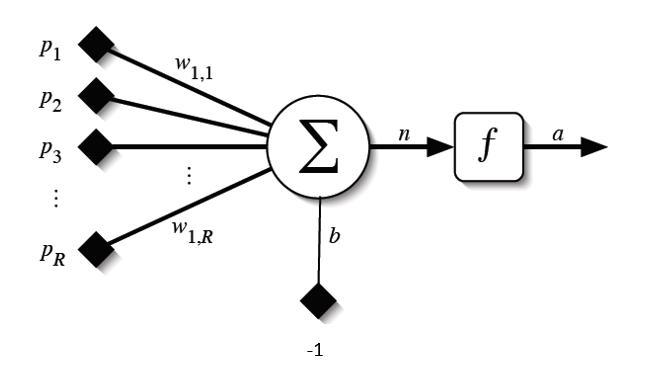
\includegraphics[width=0.6\linewidth]{fig/schemaneurone.jpg}}
  \caption{Schéma d'un neurone}
  \label{fig:neurone}
\end{figure}

Un exemple simple du réseau de neurones est la séparation d’un plan en deux.\\
Imaginons un neurone à deux entrées $e_1$ et $e_2$, chacune attribuée d’un poids $w_1$ et $w_2$. On affecte au neurone un biais $b$ et une fonction d’activation seuil (Heavyside par exemple).\\
Notre neurone renverra : 1 si $(e_1w_1+e_2w_2) - b >0$ et 0 sinon.

Si les $e_1$ et $e_2$ représentent les abscisses et ordonnées d’un point du plan, on reconnaît dans l’argument de la fonction d’activation l’équation d’une droite affine. Notre neurone pourra donc distinguer les points du plan selon le côté de la droite où ils se trouvent.

On peut déjà voir qu’une modification des poids entraînera une délimitation différente du plan. On peut donc imaginer faire « apprendre » au réseau une délimitation choisi en modifiant ses poids. Nous reviendrons sur ce concept par la suite.\\
Cependant, les applications d’un neurone seul sont vite limitées. C’est pourquoi on va s’intéresser à en connecter plusieurs entre eux.

\subsection{Réseau de neurones et perceptron} % (fold)
\label{sub:reseau_de_neurones}
On a déjà vu que le neurone se prêtait bien à une séparation binaire des données. On va voir que l’organisation de neurones en réseau permet de meilleures classifications.\\
L’organisation du réseau se fera au moyen de couches de neurones. Une couche est un ensemble de neurones possédant les mêmes entrées. Cette couche aura alors plus d'une sortie (une par neurone dans la couche), ce qui permet de généraliser aux sorties vectorielles le concept du neurone seul. En ayant ainsi une sortie vectorielle, on peut utiliser les sorties d'une couche en tant qu'entrée d'une autre couche, ce qui complexifie encore les fonctions possiblement décrites par les neurones.
On peut imaginer des réseaux plus complexes où la sortie n'est pas réutilisée dans la couche suivante mais plusieurs couches plus loin ou dans des couches antérieures. On peut en réalité construire le graphe de neurones que l'on veut, mais, dans la pratique, seules certaines structures sont utilisés. 

\begin{figure}[ht]
  \centerline{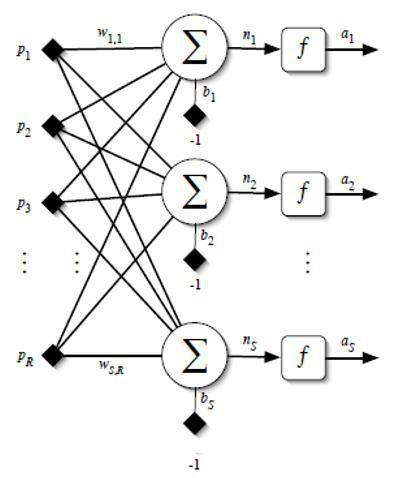
\includegraphics[width=0.5\linewidth]{fig/schemacouche.jpg}}
  \caption{Exemple d'une couche de neurones}
  \label{fig:couche}
\end{figure}

Le perceptron est un modèle de réseau de neurones auquel on va s’intéresser particulièrement. Il s'agit d'un réseau linéaire où chaque couche est entièrement connectée à la suivante, c'est-à-dire que chaque neurone d'une couche prend en entrée toutes les sorties de la couche précédente. On ne trouve aucune boucle dans le graphe d'un perceptron, c'est donc une propagation vers l'avant.
L’utilité d’avoir plusieurs couches se comprend facilement. Si on reprend notre exemple du problème de classification des points, on peut imaginer, par exemple, quatre neurones qui enverront leur sortie sur un neurone à quatre entrées. Chacun des neurones réalisera la séparation du plan en deux selon le principe déjà évoqué précédemment. Le neurone de la couche de sortie pourra réaliser facilement le rôle d’un ET logique. On vient de sélectionner un carré dans le plan. En étendant le raisonnement, on voit qu’un réseau à deux couches permet de sélectionner n’importe quelle zone convexe de l’espace des entrées (ici du plan). De même, un réseau à trois couches pourra sélectionner n’importe quelle zone concave de l’espace des entrées.

\begin{figure}[ht]
  \centerline{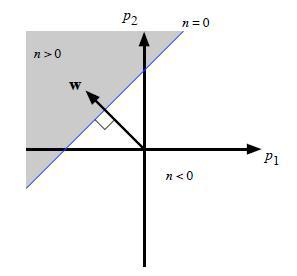
\includegraphics[width=0.5\linewidth]{fig/espace1neurone.jpg}}
  \caption{Frontière de décision pour un perceptron simple à 1 neurone et 2 entrées}
  \label{fig:espace1neurone}
\end{figure}

On appelle la dernière couche, celle qui donne le résultat du réseau de neurones, la couche de sortie; et la première couche où l'on donne les entrées est appelée couche d'entrée. Les autres couches sont appelées des couches cachées. Cette appellation vient du fait qu’a priori, nous n’avons aucun moyen de voir ou de corriger les comportements des neurones cachés. En effet, avec la seule donnée de la sortie, l’influence des poids des couches cachées sur celle-ci n'est pas évidente. C'est ce que nous allons étudier dans la partie suivante. 
% subsection reseau_de_neurones (end)




% subsection le_neurone (end)

\subsection{Apprentissage par rétro-propagation}

Il existe plusieurs types d'apprentissages du réseau. Les deux grandes catégories sont l'apprentissage supervisé et l'apprentissage non supervisé. 
Un apprentissage supervisé nécessite une base d'apprentissage à enseigner au réseau. Elle est composée d'associations entre entrées et sorties voulues. Le réseau déduira de cette base les autres cas qu'on ne lui aura pas appris. Une apprentissage non supervisé ne nécessite pas une telle base d'apprentissage.

Dans le cadre du perceptron, nous utilisons un apprentissage supervisé, la rétro-propagation des erreurs. Il s'agit en fait d'effectuer une descente de gradient. Nous avons notre réseau qui représente $F$ une fonction, cette fonction dépend de nombreux paramètres qui sont les poids $W$ de tous les neurones de toutes les couches (ainsi que les biais). Lorsque l'on veut faire tendre $F$ vers une fonction $G$, et que l'on peut avoir une distance entre ces deux fonctions, on obtient alors un problème de minimisation, avec pour paramètres d'optimisation les poids $W$. L'algorithme de descente de gradient consiste à calculer pour chaque paramètre le gradient par rapport à la sortie (c'est une descente de Newton quand on est à une dimension) afin de déplacer ce paramètre dans la bonne direction pour minimiser la sortie.

Comme dit précédemment, on n'a pas facilement accès aux couches cachées, et il parait très coûteux d'opter pour des calculs de dérivées discrètes pour obtenir les gradients voulus pour tous les paramètres.
La rétro-propagation consiste à calculer l’influence de chaque paramètre sur la sortie et à les mettre à jour en fonction de cette influence. On a vu que les couches de neurones avaient leurs propres sorties, on peut donc calculer l'influence des poids d'une couche sur sa sortie propre, puis s'en servir pour calculer l'influence sur les entrées, qui sont la sortie d'une couche précédente, on procède comme suit : 

Les paramètres que l’on fait évoluer sont les poids et les biais.
La formule de mise à jour est la suivante :
\[
W(t+1) = W(t) + \eta \frac{\partial E}{\partial W} 
\]
avec $\eta$ le pas de convergence, $\frac{\partial E}{\partial W} $ la matrice de terme général $\frac{\partial E}{\partial W_{i,j}} $.\\
Pour pouvoir mettre à jour les poids, il faut donc calculer les $\frac{\partial E}{\partial W_{i,j}} $.\\
A la couche $k$ l'influence des poids est donnée par : 
\[
	\frac{\partial E^p}{\partial W _k} = \frac{\partial F}{\partial W}(W_k, X_{k-1})\frac{\partial E^p}{\partial X_k}
\]

Avec $\frac{\partial F}{\partial W}(W_k, X_{k-1})$ la matrice jacobienne de F par rapport à la variable $W_k$.

Pour pouvoir calculer l'influence des poids de toutes les couches, il faut donc calculer $\frac{\partial E^p}{\partial W_k}$

On peut calculer par récurrence cette valeur pour toutes les couches.
\[
	\frac{\partial E^p}{\partial X _{k-1}} = \frac{\partial F}{\partial X}(W_k, X_{k-1})\frac{\partial E^p}{\partial X_k}
\]

Avec $\frac{\partial F}{\partial X }(W_k, X_{k-1})$ la matrice jacobienne de $F$ par rapport à la variable $X_k$. De plus, dans un perceptron, on peut noter la sortie de la couche $k$ : 
\[
Y_k = W_k X_k \]
\[
X_k = F(Y_k)
\]

On obtient donc ces 3 équations : 
\begin{align*}
\frac{\partial E^p}{\partial y_k^i} &= f'(x_k^i)\frac{\partial E^p}{\partial x_k^i} \\
\frac{\partial E^p}{\partial w_k^{i,j}}&= x^j_{k-1} \frac{\partial E^p}{\partial y_k^i}\\
\frac{\partial E^p}{\partial x_{k-1}^m} &= \sum_i(w_k^{im}\frac{\partial E^p}{\partial X_k})
\end{align*}

En forme matricielle, ces équations donnent :
\begin{align*}
\frac{\partial E^p}{\partial Y_k} &= Diag(f'(x_k^i))\frac{\partial E^p}{\partial x_k^i} \\
\frac{\partial E^p}{\partial W_k}&= X^T_{k-1} \frac{\partial E^p}{\partial Y_k}\\
\frac{\partial E^p}{\partial X_{k-1}} &= W_k^T\frac{\partial E^p}{\partial X_k}
\end{align*}

On obtient donc une formule de récurrence que l'on doit propager de la dernière couche à la première couche (d'où le terme rétro-propagation). On sait donc maintenant mathématiquement faire l'apprentissage d'un perceptron : il nous faut des données connues, une fonction d'erreur (appelée Loss Function dans la littérature), et appliquer cet algorithme.


\section{Conception logicielle des réseaux de neurones}
\paragraph*{} % (fold)
L'un des objectifs du projet est la conception d'une librairie permettant l'implémentation de réseaux de neurones. Notre démarche est la suivante, nous cherchons à mettre en place la structure la plus simple possible mais également la plus souple possible. Ainsi nous ne cherchons pas l'exhaustivité de notre librairie, mais nous pouvons facilement la compléter dès lors que nous avons besoin de fonctionnalité supplémentaire.

\paragraph*{} % (fold)
Notre code est structuré autour de 3 types de classes, les classes permettant la création et le fonctionnement d'un ou plusieurs réseaux de neurones (ce sont les classes qui font l'intelligence du programme, noté $brain$), les classes apportant des outils de compréhension et de travail sur les réseaux (affichage de résultats, chargement et sauvegarde de paramètres, etc) et les classes permettant de lancer une expérience (classes $main$, instanciant les objets et les expériences).

Le projet est découpé en 2 répertoire Github, le premier correspondant au code le plus simple, fonctionnel sur le problème du XOR, le second correspondant au développement suivant. Ces derniers développement correspondent à la généralisation à tout types de problèmes d'apprentissage de perception simple, puis à la mise en place du GAN et toutes les évolutions que nous avons mis en place.

Vous pouvez retrouver les codes sur https://github.com/Supelec-GAN/Salamandre-XOR.git et sur https://github.com/Supelec-GAN/Salamandre-Code.git .

\subsection{Structure du code} % (fold)
\label{sub:structure_du_code}

Afin de pouvoir implémenter facilement les calculs matriciels obtenus plus tôt, nous définissons notre plus bas niveau d'intelligence par une classe NeuronLayer représentant une couche de neurone. \\

Une couche de neurones est définie par sa matrice de poids $weights$, son vecteur de biais $biais$ ainsi que sa fonction d'activation $activation\_function$, nécessairement commune à tous les neurones dans cette structure.

\paragraph{Présentation des méthodes} % (fold)
 \label{par:presentatation_des_methodes}
 
 \begin{itemize}
 	\item $compute$ : Propagation d'une entrée au sein de cette couche.
 	\item $backprop$ : Rétro-Propagation de l'influence de l'erreur de la sortie de la couche avec mise à jour des poids et calculs de l'influence de l'erreur sur la sortie.
  \item $derivate\_error$ : Calcul intermédiaire dans la rétro-propagation.
  \item  $init\_derivate\_error$ : Calcul de la dérivée de l'erreur pour la couche de sortie
 \end{itemize}

Pour faire nos réseaux de Neurones, nous utilisons une classe Network qui permet de relier les différents NetworkLayer. Ainsi elle possède \emph{self\_layer\_list} qui est une liste de NetworkLayer. Les méthodes principales sont :  
 \begin{itemize}
  \item $compute$ : Propagation depuis l'entrée au sein de toutes les couches.
  \item $backprop$ : Rétro-Propagation de l'influence de l'erreur de la sortie du réseau et itération de \emph{backprop} sur chaque NetworkLayer.
  \item $reset$ : Remet tout les NetworkLayer à l'état initial.
 \end{itemize}
 % paragraph presentatation_des_methodes (end) 

Afin de simplifier l'utilisation des fonctions au sein de nos réseaux, nous créons une classe Function. Elle comprend les fonctions d'activations, les fonctions d'erreur, mais également des fonctions d'apprentissage i.e. les sorties attendues pour une entrée lors de l'apprentissage (ex : XorTest renvoie le résultat du XOR, MnistTest renvoie le label pour une image labellisée donnée).

Finalement pour utiliser et interpréter des réseaux, nous avons une classe Interface, celle si comporte plusieurs méthodes importantes. $learning\_manager$ permet d'organiser l'apprentissage et la récupération de données. Elle contient également des méthodes pour afficher des résultats.


\begin{figure}[ht!]
  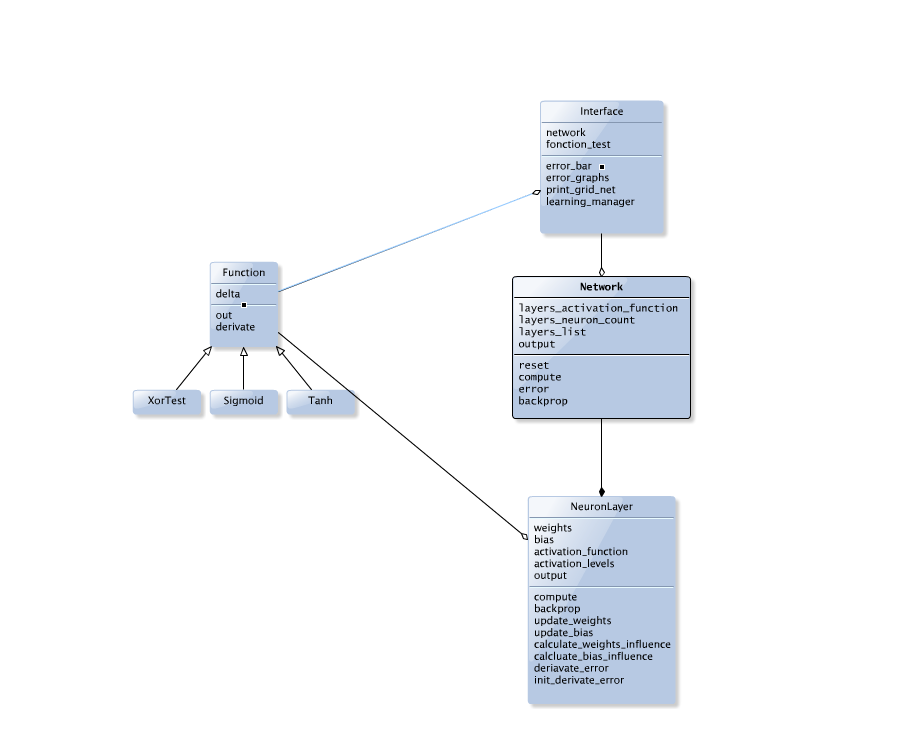
\includegraphics[width=\linewidth]{fig/uml_xor}
  \caption{Diagramme UML du code minimal et initial}
  \label{fig:uml_xor}
\end{figure}

Après évolution du code, on trouvera dans DataProcessor des méthodes pour effectuer des calculs sur les données, tels que la moyenne sur plusieurs séries d'expérience et l'écart-type. La classe DataInterface sert à la sauvegarde des résultats et des paramètres ainsi qu'à leur chargement pour utilisation ultérieure. 

Finalement les scripts run.py et tests.py servent à lancer des expériences en utilisant la librairie mise en place.

% subsection structure_du_code (end)



\section{Application au problème du XOR}

\paragraph*{}
Lorsque l'on souhaite travailler sur des algorithmes d'apprentissage par ordinateur, il est recommandé de les essayer sur des problèmes connus afin d'en vérifier les performances. \\
Le problème du XOR est l'un des plus classiques car il apporte de nombreuses difficultés.

L'objectif du XOR est de séparer le plan complexe en quatre cadrants, $(x >0, y > 0)$, $ (x>0, y<0)$, $ (x<0, y>0)$ et $ (x>0, y<0) $. Pour l'expérimentation, on restreint le plan à $[-1;1]^2$. Les sorties attendues par le réseau de neurones sont alors 1 pour les points tel que $x*y > 0 $ et -1 pour les points tels que $x*y<0$. \\
Le premier intérêt de ce problème est qu'il est non linéaire. Cela se traduit par le fait qu'une droite séparant le plan en 2 ne répond pas du tout au problème.

C'est en se basant sur la résolution du XOR que nous avons construit notre structure de réseau et vérifié la cohérence de notre code. La littérature propose comme réseau le plus simple pour ce problème une couche cachée de 2 neurones, avec 2 entrées ($x$ et $y$) et 1 sortie dans $[-1, 1]$. Nous avons étudié également quelques autres formes de réseaux pour comparer les résultats.

\paragraph{Notion de résultats} % (fold)
\label{par:notion_de_resultats}
La notion de résultats nécessite d'être correctement définie afin de pouvoir être interprétée correctement, en particulier pour la comparaison à d'autres résultats obtenus par nous-même ou par d'autres personnes. \\
La structure de perceptron sous cette forme classe les objets que l'on donne en entrée. Généralement, le résultat est défini par rapport à un pourcentage de succès dans cette classification. Pour l'obtenir, on commence par définir une erreur relative, c'est-à-dire une distance entre la sortie cible et la sortie obtenue. Un seuil est alors appliqué afin de définir une sortie booléenne de la classification de l'entrée.\\
Dans le cas du XOR, on met en place un seuil de 0.5, c'est à dire que, si l'erreur est inférieure à 50\%, le réseau a raison. Cela peut s’interpréter comme suit : le réseau donne un résultat qui indique sa confiance dans la sortie. 1 ou 0 si il est certain que la sortie doit être 1 ou 0, 0.5 si il ne peut départager l'un ou l'autre, le seuil consiste à dire que sa réponse est celle en qui il a le plus confiance.\
On cherche également à évaluer la vitesse d'apprentissage. Ainsi, on calcule le pourcentage de succès du réseau à intervalles réguliers au cours de l'apprentissage. Les réseaux étant soumis à une forte composante aléatoire (l'ordre d'apprentissage, ainsi que l'initialisation des poids), on effectue des apprentissages dans les mêmes conditions plusieurs fois afin d'obtenir des courbes moyennes, et des intervalles de confiances justifiant nos résultats.
% paragraph notion_de_résultats (end)

\paragraph{Réseau en $2\rightarrow2\rightarrow1$} % (fold)

Les résultats obtenus au début sur ce réseau extrêmement simple semblaient tout à fait aléatoires et nous ont permis de détecter des erreurs de traduction des équations de rétro-propagation en code Python. Nous avons finalement pu obtenir des résultats satisfaisants, comme le montre la figure \ref{fig:2_2_1}. 

\begin{figure}[ht!]
  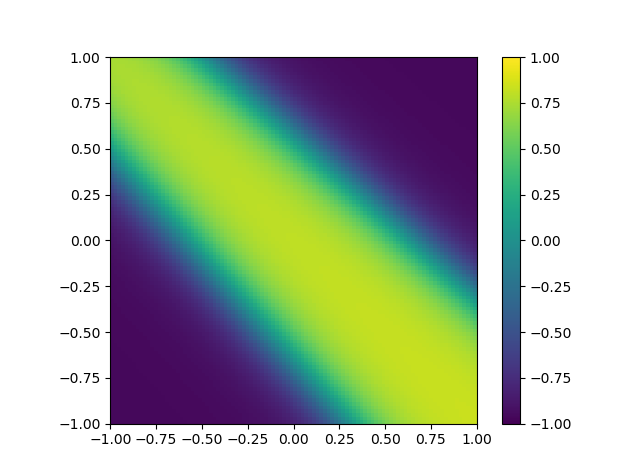
\includegraphics[width=\linewidth]{fig/xor221_eta009.png}
  \caption{Application d'un réseau 2-2-1 au plan pour xor}
  \label{fig:2_2_1}
\end{figure}


% paragraph réseau_en_2_2_1 (end)

\paragraph{Importance du pas d'apprentissage $\eta$}

L'un des paramètres de la descente de gradient est le pas d'apprentissage $\eta$. Il intervient dans le formule de mise à jour des poids :
\[
W(t+1) = W(t) + \eta \frac{\partial E}{\partial W} 
\]
Plus il est petit, plus l'algorithme avancera lentement. Cependant, s'il est trop grand, l'algorithme ne se rapprochera pas du minimum mais divergera. Il faut donc le choisir suffisamment petit pour que cela converge mais suffisamment grand pour que ce ne soit pas trop lent. La figure \ref{fig:2_2_2_1} montre en 10000 apprentissages le résultat d'un réseau entraîné sur XOR selon le pas d'apprentissage. On remarque notamment que, lors qu'il est trop élevé, le réseau n'arrive pas à découper l'espace.

\begin{figure}[ht!]
  \centering
  \begin{subfigure}[b]{.3\linewidth}
    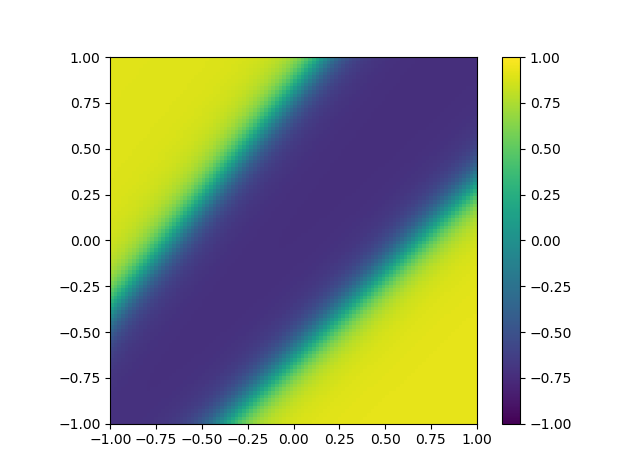
\includegraphics[width=\linewidth]{fig/xor2221_eta01.png}
    \caption{eta =0.1}
  \end{subfigure}
  \quad
  \begin{subfigure}[b]{.3\linewidth}
    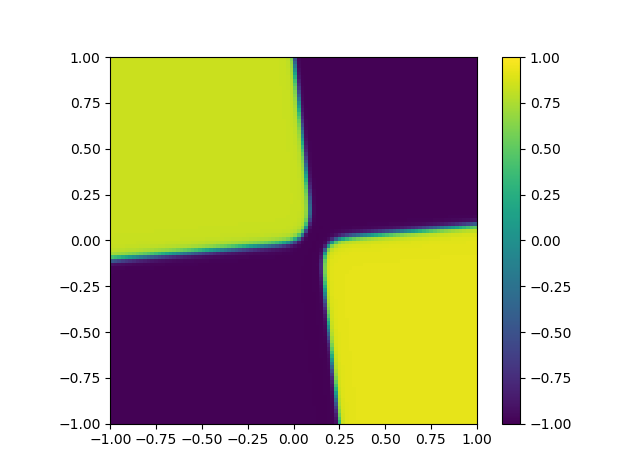
\includegraphics[width=\linewidth]{fig/xor2221_eta05.png}
    \caption{eta =0.5}
  \end{subfigure}
  \quad
  \begin{subfigure}[b]{.3\linewidth}
    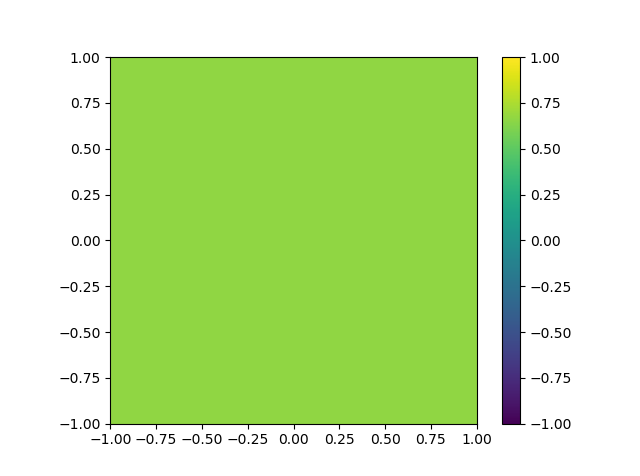
\includegraphics[width=\linewidth]{fig/xor2221_eta09.png}
    \caption{eta =0.9}
  \end{subfigure}
  \caption{Xor en 2-2-2-1 avec différents pas d'apprentissages au bout de 10000 apprentissages}
  \label{fig:2_2_2_1}
\end{figure}

\paragraph{Structure du réseau}
	La structure du réseau choisie est également importante. Comme expliqué plus haut, si le réseau est 2-2-1, il ne peut pas délimiter l'espace comme on le souhaite. Cela signifie que, pour la fonction XOR avec laquelle on travaille (à savoir qu'on représente VRAI par 1 et FAUX par -1), il ne peut pas découper le plan selon les axes des abscisses et ordonnées. En revanche, il va essayer de le délimiter de façon à accorder aux points (1,1) et (-1, -1) la valeur VRAIE et (1,-1) et (-1,1) la valeur FAUX. Pour cela, il trace une bande comme sur la figure \ref{fig:struct221}. En effet, il y a priorité sur ces valeurs puisque la base d'apprentissage de notre réseau est constituée de couples de -1 et de 1.
	
\begin{figure}[ht!]
  \centering
  \begin{subfigure}[b]{.3\linewidth}
    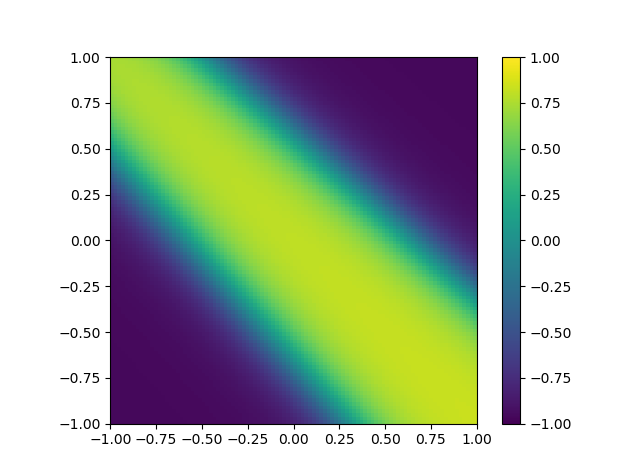
\includegraphics[width=\linewidth]{fig/xor221_eta009.png}
    \caption{Structure 2-2-1}
    \label{fig:struct221}
  \end{subfigure}
  \quad
  \begin{subfigure}[b]{.3\linewidth}
    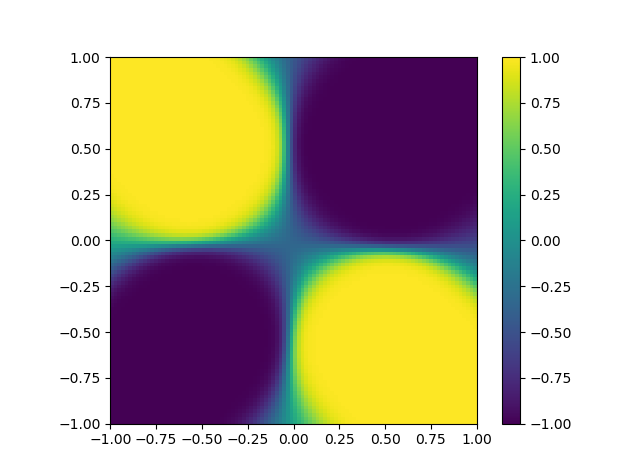
\includegraphics[width=\linewidth]{fig/xor241_eta016.png}
    \caption{Structure 2-4-1}
    \label{fig:struct241}
  \end{subfigure}
  \quad
  \begin{subfigure}[b]{.3\linewidth}
    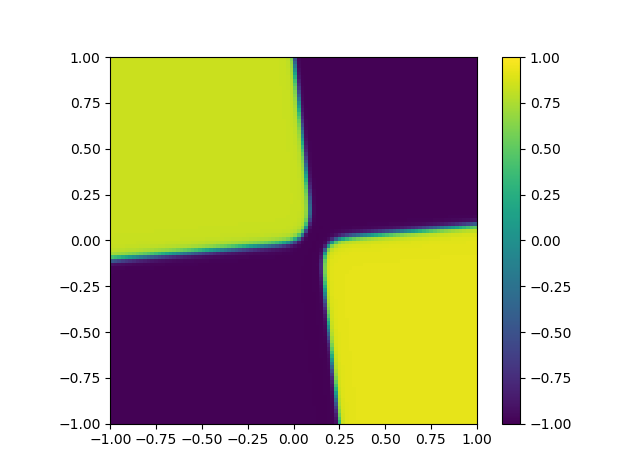
\includegraphics[width=\linewidth]{fig/xor2221_eta05.png}
    \caption{Structure 2-2-2-1}
    \label{fig:struct2221}
  \end{subfigure}
  \caption{Xor avec différentes structures}
  \label{structxor}
\end{figure}

Cependant, lorsqu'on lui accorde plus de neurones, 4 neurones sur la première couche comme sur la figure \ref{fig:struct241}, ou 3 couches par exemple comme sur la figure \ref{fig:struct2221}, le réseau découpe l'espace comme souhaité. En revanche, le XOR avec la structure 2-2-2-1 est assez instable : pour les mêmes paramètres, on peut obtenir un réseau qui converge et un autre qui se plante complètement comme le montre la figure \ref{fig:2_2_2_1_instable}
	
\begin{figure}[ht!]
  \centering
  \begin{subfigure}[b]{.4\linewidth}
    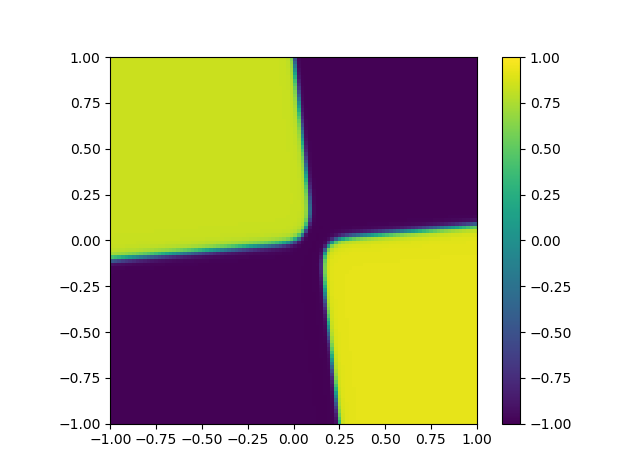
\includegraphics[width=\linewidth]{fig/xor2221_eta05.png}
    \caption{XOR qui converge}
    \label{fig:_05}
  \end{subfigure}
  \quad
  \begin{subfigure}[b]{.4\linewidth}
    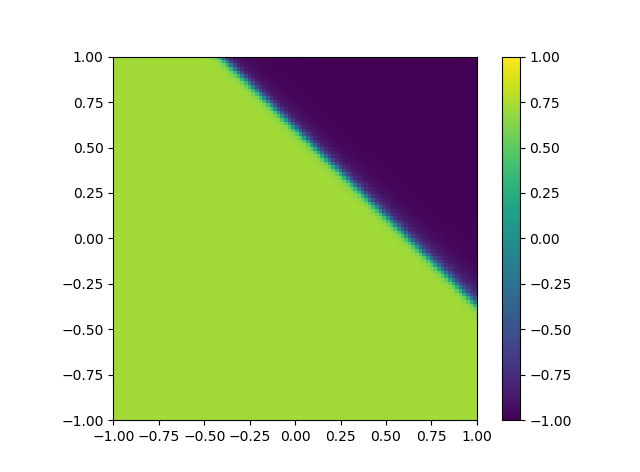
\includegraphics[width=\linewidth]{fig/xor2221_eta05v2.png}
    \caption{XOR planté}
  \end{subfigure}
  \caption{XOR en 2-2-2-1 avec eta =0.5}
  \label{fig:2_2_2_1_instable}
\end{figure}

\paragraph{Conclusion sur le XOR} % (fold)
\label{par:conclusion_sur_le_xor}
Pas d'apprentissage très petit par rapport à la littérature\\
Influence des fonctions d'activation
% paragraph conclusion_sur_le_xor (end)

\section{Application à la base de données MNIST}

\subsection*{Description du problème} % (fold)

Pour le problème du MNIST qui consiste à apprendre à reconnaitre des chiffres manuscrits, les données étaient les suivantes : 
\begin{itemize}
	\item 60000 images pour l’apprentissage, avec leurs étiquettes
	\item 10000 images de test
\end{itemize}

Toutes les images ont une dimension de 28*28 pixels en noir et blanc. Ces sets d’images sont récupérables sur le site http://yann.lecun.com/exdb/mnist/ sous le format IDX. L’extraction de ce format vers une liste python est faite grâce au module python-mnist.

\subsection*{Paramètres généraux utilisés :} % (fold)
Les fonctions d’activation utilisées pour toutes les expériences ici sont des sigmoïdes de paramètre $\mu$ : 
$\sigma_\mu(x) = \frac{1}{1+e^{-\mu x}}$\\
On pourra étudier l’influence de $\mu$ sur la vitesse de convergence.
Puisque les fonctions d’activation utilisées sont des sigmoïdes dont la sortie est dans [0, 1], les valeurs d’entrées situées entre 0 et 255 sont normalisées entre 0 et 1.\\
L’erreur utilisée sur la couche de sortie est l’erreur quadratique.\\
Les poids sont initialisés avec une répartition gaussienne centrée réduite. Les biais sont initialisés à 0.\\
De bons résultats ont été obtenus avec le réseau suivant, conformément à la littérature :
\begin{itemize}
	\item Eta 0.2
	\item Sigmoïde 0.1
	\item Réseau à une couche cachée de 300 neurones et 10 neurones de sortie (784-300-10)
	\item Apprentissage stochastique
\end{itemize}
Avec ce type de réseau, on obtient rapidement des taux de succès proche de 95\% après 10 passes de l’ensemble du set d’apprentissages, et un écart-type final de 0.001223411. Nous allons maintenant voir l’influence des différents paramètres.

\begin{figure}[ht!]
  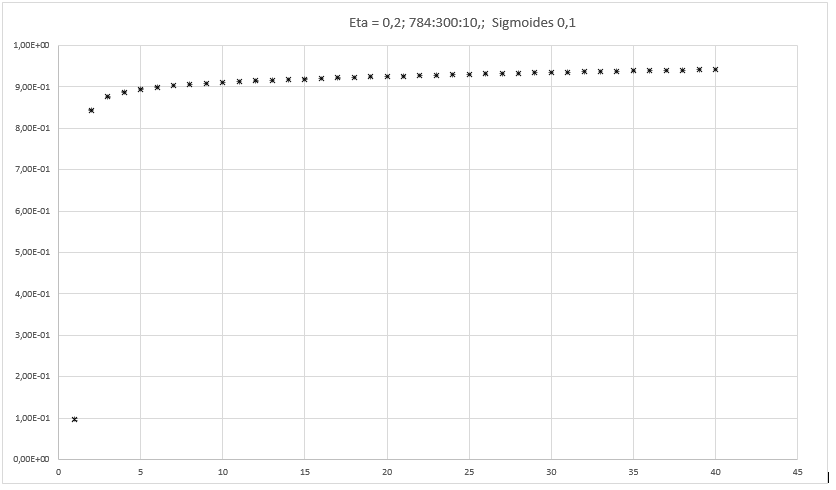
\includegraphics[width=\linewidth]{fig/MNIST_result_1.png}
  \caption{Courbe de réussite du réseau sur MNIST}
  \label{fig:mnist_result_1}
\end{figure}

\subsubsection*{Variation d’êta :}


Sur le réseau 300-10 précédent, une augmentation du êta de 0.2 à 10 ne semble qu’améliorer la vitesse de convergence comme le montre la figure \ref{fig:mnist_influence_eta}. 
L’écart-type n’augmente pas et on obtient une meilleure précision à la fin.

\begin{figure}[ht!]
  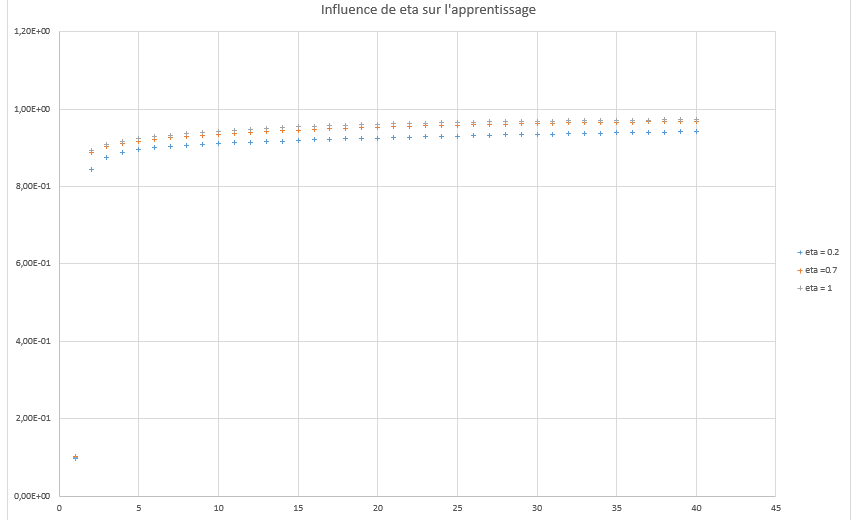
\includegraphics[width=\linewidth]{fig/MNIST_influence_eta.png}
  \caption{Courbe de réussite du réseau sur MNIST avec différents $\eta$}
  \label{fig:mnist_influence_eta}
\end{figure}

\subsubsection*{Choix du paramètre de la sigmoïde :}
Ici, l’influence du choix de la sigmoïde est observée. Les tests ont été effectués avec $\mu = 0.1$ et $\mu = 0.5$ comme paramètre de sigmoïdes.
[[insert courbe (cf 17/01/18)]]
On remarque qu’en tout point, choisir 0.1 en paramètre à la place de 0.5 est mieux : vitesse de convergence, précision finale, écart-type. Ce résultat empire avec un êta plus élevé, au point de ne plus réussir à apprendre. On restera donc sur une sigmoïde de paramètre 0.1 pour la suite des expériences.

\begin{figure}[ht!]
  \centering
  \begin{subfigure}[b]{.5\linewidth}
    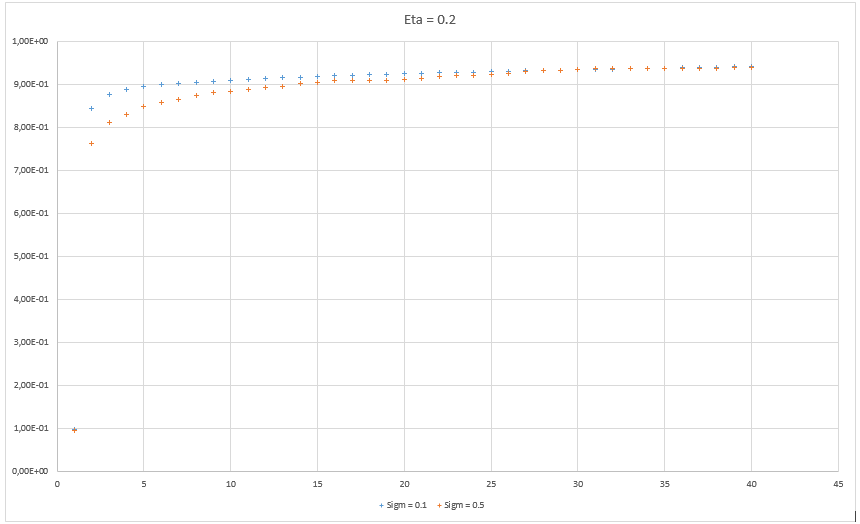
\includegraphics[width=\linewidth]{fig/MNIST_inflsigm_eta02.png}
    \caption{$\eta=0.2$}
  \end{subfigure}
  \quad
  \begin{subfigure}[b]{.5\linewidth}
    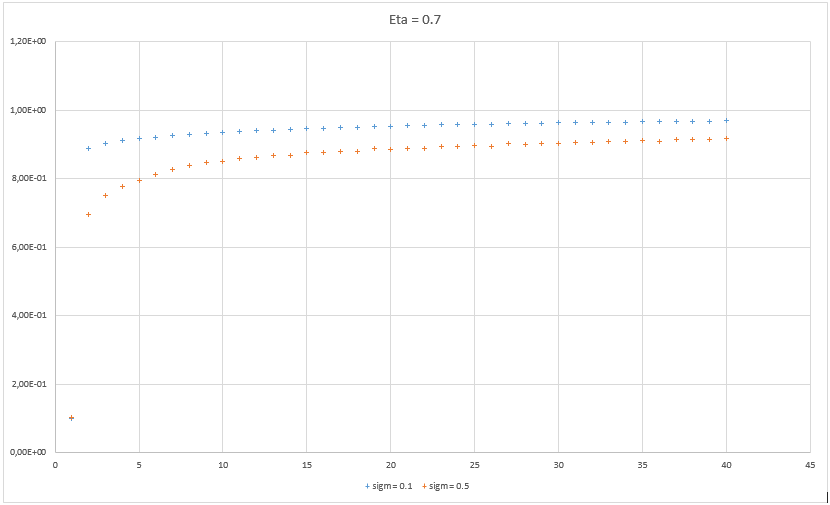
\includegraphics[width=\linewidth]{fig/MNIST_inflsigm_eta07.png}
    \caption{$\eta=0.7$}
  \end{subfigure}
  \begin{subfigure}[b]{.5\linewidth}
    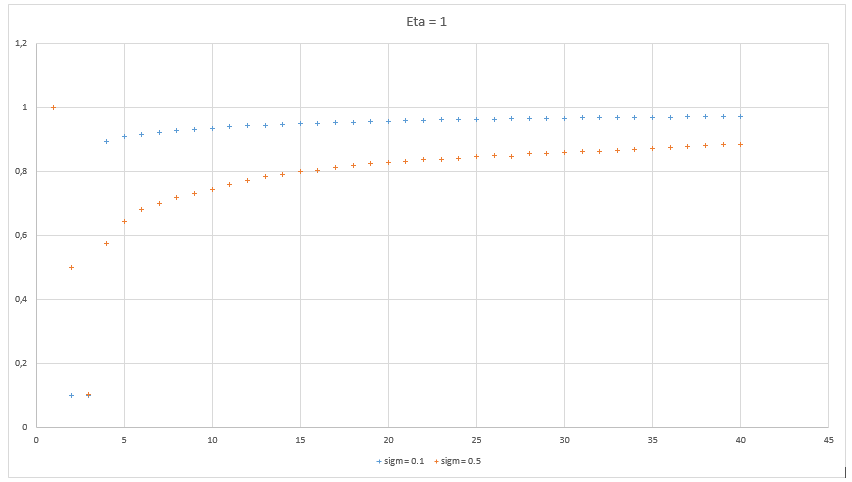
\includegraphics[width=\linewidth]{fig/MNIST_inflsigm_eta1.png}
    \caption{$\eta=1$}
  \end{subfigure}
  \caption{Comparaison de deux sigmoïdes pour plusieurs $\eta$}
  \label{fig:MNIST_inflsigm}
\end{figure}

\subsubsection*{Différents réseaux :} 
Intuitivement, un réseau avec plus de couches cachées devrait obtenir une meilleure précision, mais devrait avoir un temps d’apprentissage plus long. Ces résultats se confirment avec des expériences sur le réseau à une couche cachée (300 neurones) précédent, et un réseau sans couche cachée. Ce dernier converge très vite aussi bien vis-à-vis du nombre d’apprentissages nécessaire que du temps de calcul. Cependant, il est difficile de dépasser les 90\% de succès. Alors que sur le réseau avec couche cachée, on arrive à obtenir moins de 5\% d’erreur. En revanche, les temps de calculs sont plus élevés. Le réseau avec deux couches cachées, 1000 puis 300, a aussi été testé. Les résultats ici sont satisfaisants, cependant l’amélioration des résultats n’est pas très importante, alors que les temps de calculs augmentent fortement.
[[insert courbe (cf 17/01/18)]]
Ce problème est bien connu dans l'étude des réseaux de neurones, et a justifié l'apparition de l'apprentissage profond, que nous évoquerons plus tard.
Temps de calcul approximatifs pour une passe du set d’apprentissage, et un test tous les 1000 apprentissages :
\begin{itemize}
	\item 5-6 minutes pour le 784-1000-300-10
	\item 4 minutes pour le 784-300-10 
\end{itemize}
Ces temps peuvent être améliorés avec l’introduction du batch learning qui permet de calculer les résultats des tests plus rapidement.
%!TEX root = main.tex
% \begin{figure}[htb]
% \begin{center}
% %optional pour enlever un peu d'espace blanc de votre silhouette
% %\vspace{-.3cm}
%  %\includegraphics[keepaspectratio,width=0.5\textwidth]{fig/nomde}
% % analoog
% %\vspace{-0.6cm}
%  % \caption{ici un logo}
%  % \label{fig:ruglogo}
% %analoog
% %\vspace{-.6cm}
% \end{center}
% \end{figure}

% Utilisation du template
% \cite(reference à citer)
% \ref(figure à référencer)

%\bibliography{reference}

\chapter{Generative Adversarial Networks}

\paragraph{}
	La première partie de cette étude nous a permis de maîtriser l'utilisation de réseaux en perceptron et de structurer une architecture logicielle efficace et souple pour l'étude des GAN. \\
	Après avoir obtenu des résultats satisfaisants dans la classification de motif sur la base MNIST, nous étudions la génération de données à l'aide de réseaux de neurones en nous basant sur le concept de GAN, introduit par I. Goodfellow en 2016 \cite{nips-2014}.\\
	Notre objectif dans cette partie est d’appréhender le concept de GAN et de l'appliquer sur notre programme afin d'étudier les différents paramètres. 
\section{Principe}
	\paragraph{}
		Le GAN s'inscrit dans les problèmes de générations de données par ordinateurs. Ses modèles cherchent à produire de données nouvelles respectant un certain nombre de contraintes. Les applications possible sont très nombreuses, tant au niveau scientifiques qu'industrielles, avec par exemple la modélisation de nouvelles protéines, le dessin de circuit intégrés, etc. 
		Le but de nos GAN sera de générer des images que l’on ne pourra distinguer de « vraies » images, prises avec un appareil photo.\\

		Le principe général est le suivant : \\ un GAN est constitué de deux réseaux de neurones, le Générateur (G) et le Discriminateur (D). Le Générateur a pour but de créer les images et le Discriminateur de déterminer si les images qu’on lui donne sont de « vraies » images ou ont été créées par le Générateur. Ces deux réseaux sont mis en compétition : le Générateur a pour but de tromper le Discriminateur tandis que le Discriminateur doit détecter les « fausses » images.\\
		L’apprentissage du Discriminateur se fait à la fois sur des images générées par le Générateur et de « vraies » images, issues d’une banque d’images afin de continuellement améliorer sa capacité de discernement.\\
		L’apprentissage du Générateur dépend de la réponse du  Discriminateur : lorsqu’il génère une image, on la donne au Discriminateur pour voir si le Générateur a réussi à le tromper. Le discriminateur sert donc de fonction d'erreur au Générateur.

	\paragraph{}
		De façon plus formelle, on travaille avec 3 distributions : $p_x$, la distribution idéale des vraies images, $p_{data}$, la distribution de l'échantillon des vraies images et $p_{model}$ la distribution réalisée par les images issues du Générateur. Le but de l’apprentissage est de rapprocher $p_{model}$ de $p_x$. Comme $p_x$ nous est inconnu, on va plutôt s'approcher de $p_{data}$.\\
		On dispose de deux fonctions de coûts $J_D(\theta_G, \theta_D)$ et $J_G(\theta_G, \theta_D)$, représentant respectivement les fonctions de coûts du Discriminateur et du Générateur. On note $\theta_G$ et $\theta_G$ les paramètres des réseaux. Les fonctions de coûts dépendent bien des paramètres des deux réseaux car le Discriminateur apprend à discerner les vrais images des fausses, dépendantes du générateur, et le générateur apprend via le résultat du Discriminateur.\\ C'est un problème d'optimisation simultanée. 
		Il peut également être décrit comme un problème de jeux à informations complètes. G à accès aux données de D, mais ne peut influer que sur $\theta_G$ et D à accès aux données de G, mais ne peut influer que sur $\theta_G$. Cette vision permet de déduire un algorithme ou chaque joueur va faire un mouvement de manière optimal, afin de tendre vers un équilibre de Nash.

\section{Apprentissage}

	\paragraph{}
		L’apprentissage consiste à appliquer cette méthode de jeu à l'apprentissage des réseaux de neurones.
		Nous fournissons au Discriminateur des images $x$ (de la BDD MNIST par exemple) et lui demandons de nous renvoyer un réel entre 0 et 1, qui représente son degré de confiance sur le fait que l’image fournie ai été tirée d’une banque de donnée authentique ou du Générateur. Les réponses attendus sont respectivement ($D(x) = 1$) et ($D(x) =0$) ce qui nous permet de calculer des erreurs pour la descente de gradient du Discriminateur.\\ 
		Le Générateur, quant à lui, génère une image à partir d’un vecteur de bruit $z$. Cette image est ensuite jugée par le Discriminateur : $D(G(z)) = 1$ si le Générateur a dupé le Discriminateur et 0 sinon. L'objectif du Générateur est d'être le plus proche possible de la première situation, l'erreur pour la descente du gradient du Générateur en est déduite.\\
		L'apprentissage complet se fait en alternant les 2 phases successivement, chaque réseau jouant tour à tour. On parle de réseau concurrent car le Discriminateur cherche à obtenir $D(G(z)) = 0 $ pour tout $z$ et le Générateur $D(G(z)) = 1$.

	\paragraph*{Problèmes liés à la convergence}
		L'apprentissage des GANs n'est pas simple à maitriser car ils ne fonctionnent pas comme un seul réseau qui apprend avec une algorithme de descente de gradients. Il s'agit en réalité d'une descente de gradient simultanée ($J_G \text{ et } J_D$) qui n'est pas un cas particulier, mais une généralisation du problème classique d'optimisation. La résolution mathématique de ce problème n'est pas trivial, et les méthodes ne s'adaptent pas facilement aux réseaux de neurones. La méthode proposé si dessous est donc une heuristique que l'on peut fortement adapter. Elle a fait ses preuves dans de nombreux cas, malgré son manque d’appui mathématique. Cependant d'autres façon de voir les choses permettent d'obtenir des résultats toujours corrects mais avec une plus grande rigueur. Les questionnements mathématiques seront abordés dans les axes de recherches.  

\section{Paramètres des GANS}

	Voici une description des paramètres principaux sur lequel on peut jouer pour l'implémentation d'un GAN. Ils sont nombreux car la description précédente est en réalité peu restrictive.

	\begin{itemize}
	 	\item Fonctions de coûts
	 	\item Ratios d'apprentissage
	 	\item Paramètres classiques des réseaux de neurones (Structures des réseaux, pas d'apprentissage, etc.)
	\end{itemize}


\section{Structure et utilisation du code}
	{description des modifications importantes pour le GAN (or optimisation du code source)}


\section{Premier résultats pour des GANs simples}
	Afin d'appréhender correctement le fonctionnement des GANs, il est nécessaire de tester de nombreux paramètres. Les résultats, fructueux ou non, permettent d'évaluer l'intérêt des paramètres et de comprendre le sens "physique" de leur influence.\\
	Ces essais se feront sur la base MNIST, c'est-à-dire que notre objectif sera d'obtenir par le générateur des chiffres manuscrits qu'il aura dessiné par lui-même. Plus précisément on attend du générateur après apprentissage que chaque entrée génère un chiffre entre 0 et 9 qu'un être humain ne peut distinguer d'un chiffre manuscrit écrit par un humain (donc de la base MNIST).

	\subsection{Méthodologie initiale}
		L'un des objectifs de ce projet est de décortiquer au mieux la méthode GAN. Pour cela nous utilisons les réseaux de neurones les plus simples, ils seront complexifiés par la suite. La plupart des articles sur le sujet présentent des réseaux utilisant des structures avancés (couche convolutive, optimiseur de descente, etc.) il n'est donc pas possible de se référer aux paramètres de ses articles pour obtenir immédiatement des résultats et s'assurer que notre programme tourne correctement. \\
		Pour le choix du réseau Discriminateur, le choix se porte sur des structures ayant eu de bonnes performance pour le MNIST, c'est-à-dire soit un très bon taux final, soit une vitesse de convergence élevée. En effet le Discriminateur n'est qu'un simple classificateur sur la base MNIST. Le choix du générateur est plus complexe car il faut que la structure soit assez puissante pour dessiner des chiffres. Cela semble bien plus difficile que simplement les reconnaitre, car ils peuvent être reconnus à l'aide de features très particulières, tandis que la génération exige une information complète. La première idée pour dimensionner le réseau est d'avoir une entrée suffisante pour générer la diversité de sortie souhaité, mais pas nécessairement plus pour ne pas avoir un réseau trop lourd en calcul.\\
		Pour les autres paramètres, aucune idée précise de leurs ordre de grandeur nécessaire, en particulier le pas d'apprentissage (très différents pour MNIST et XOR par exemple).\\
		Nous avons donc balayé les paramètres possibles afin d'obtenir le maximum d'information avec des GANs simples.//
		Le principal soucis que nous avons eu avec cette approche fut l'évaluation des performances de nos GANs, au début de l'étude, alors que nous n'arrivions pas encore à former des chiffres satisfaisants, nous n'avions aucun moyen pour savoir si un paramètre était meilleur qu'un autre. //
		Nous avons considéré l'étude de l'évolution des scores que le Discriminateur attribuait aux images de Mnist et à celles du Générateur, mais elles se sont révélées inexploitables : le score brut ne permettait pas de rendre compte de l'apprentissage effectué jusqu'alors. Et le score ne révélait en rien la qualité de l'image. 
{ici des exemples de courbes sur lesquelles on travaillait au début } 




\section{Mode Collapse}
	\subsection{Présentation du problème}
		Le problème du Mode Collapse est bien connu dans la confections de GANs. Il se traduit par un générateur qui ne produit plus qu'un type de données particulier, sans diversité. 
		Imaginons un générateur qui doit générer deux types de données : X et Y. Après quelques apprentissages, il réussit à générer des X suffisament convaincants pour tromper le Discriminateur. A ce moment, le Générateur est "récompensé" pour tromper Le Discriminateur, et ce dernier n'arrive plus à distinguer les X de la BBD de ceux générés artificiellement. Du coup le Discriminateur ne fait plus confiance aux X qu'il reçoit et se concentre sur les Y, sur lesquels il se fait davantage récompenser pour son travail. Après quelques apprentisasges à nouveau, le générateur oublie les X et se met à générer des Y trompeurs.
		Ainsi, notre GAN fournit alternativement des X et des Y médiocres sur une longue periode, alors qu'au contraire on souhaiterai obtenir des données diverses.
	\subsection{Une première idée de résolution du problème}
		Une première étape pour éviter le problème est décrite dans l'article de NIPS 2014 de I.Goodfellow \cite{nips-2014}. Il s'agit d'ajouter du bruit sur une couche intérmédiaire du Générateur. En forçant ainsi une part d'aléatoire dans le Générateur, on peut éspérer qu'il ne se "vérrouille" pas à produire une donnée particulière. 
		Nous avons implémenté cette solution lors de notre travail sur MNIST. Goodfellow suggère plusieurs techniques d'implémentations : ajouter un bruit à la sortie d'une couche, mutiplier le vercteur de sortie terme à terme avec un vecteur de bruit, ou encore concaténer le vecteur de sortie avec un vecteur de bruit gaussien. Nous avons chosi d'implémenter cette dernière solution. On pourrait toujours craindre que dans le pire des cas, le Générateur décide d'atribuer au bruit des poids nuls ou négligeables. Mais lors de l'implémentation, on a néanmoins remarqué une baisse significative du taux de Mode Collapse dans nos expériences.
		\subsection {Perturber le GAN avec des "secousses" } 
		Une approche pour empêcher le GAN de tomber en Mode Collapse fut suggérée par T. Salimans. Elle consiste en ajouter une part d'aléatoire dans le processus. //
	Plutôt que de s'attendre à ce que le Discriminateur renvoie 1 sur une image de la base de données, on calcule l'erreur à partir d'un réel proche de 1 (entre 0.7 et 0.99) afin de plus facilement le récompenser. //
	En parallèle, de temps en temps (un cas sur deux cent, grand maximum ) on trompe le Discriminateur en lui disant qu'on attendait une vraie image lorsqu'il en traite une fausse et inversement. //
	Ces deux techniques permettraient, en théorie de renforcer le générateur de manière subtile (pour la première ) et de le perturber suffisamment pour sortir des situations de Collapse (deuxième technique ) //
	Cependant, les expériences menées par nos soins sur ces techniques ne se sont pas montrées concluantes, le Collapse apparaissait parfois plus vite que sans ses techniques . //
	Cela est sans doute dû au fait que nos GANs, contrairement à ceux de Goodfellow et Salimans, n'étaient pas assez robustes pour qu'on puisse se permettre d'ajouter cette part d'aléatoire. 
	
	

	\subsection{Une autre piste : le minibatch}
		Une autre methode déstinée à empécher le Mode Collapse et à forcer la diversité des données générées fut proposée par T.Salilmans et I.Goodfellow dans Improved techniques for training GANs \cite{salimans_improved_2016}.\\
		L'idée consiste en proposant au Discriminateur non plus une seule donnée du Générateur mais bien tout un petit paquet (minibatch). Une distance mathématique entre chacune des données de ce minibatch est calculée et traitée (passée à l'exponentielle négative) puis ajoutée à la sortie d'une couche intermédiaire du Discriminateur. //
		Ainsi, on envoie $n$ images dans notre Discriminateur, qui possedera sur une couche intermédiaire $n$ neurones suplémentaires, l'activation du neurone $i$ correspond à un score de ressemblance entre la donnée traitée actuellement et la donnée $i$. Le Discriminateur a donc un moyen de determiner si les données générées par le Générateur sont toutes semblabes entre elles ou non. Il pourra ainsi facilement punir le Discriminateur si celui tombait en Mode Collapse . //
		
	



\section{Résultat sans collapse}
{même chose que la section premiers résultats, mais avec le bruit en entrée}
\section{Autres problèmes rencontrés } 
Comme mentionné plus haut, il nous a été très difficile de savoir dans quel direction progresser.//
En effet, il n'existe pour l'instant aucune méthode fiable pour attribuer un "score de vraisemblance "  aux donnés générées par GAN. En l'état, la meilleure méthode suggérée par l'état de l'art consiste à demander à des humains si les chiffres qu'on leur présentait leur paraissaient vraisemblables ou non. L'expérience fur tentée par Goodfellow avec l'aide du captcha d'Amazon, mais même de tels moyens n'ont pas donnés de résultats très satisfaisants (il se trouve que le sujet humain, à l'instar d'un Discriminateur, apprenait de ses erreurs et devenait trop bon trop vite ) . //
On a donc recherché un moyen d'évaluer nos résultats. Après qu'on nous ait suggéré des pistes sur le traitement d'images, nous nous sommes tournés vers le WGAN, dont on parlera plus tard , qui ne souffrait pas de telles difficultés . 

De plus, après un bref entretien avec Ian LeCun, (où nous avons constaté que nous butions sur des problèmes biens établis de la théorie du GAN), une autre piste d'amélioration a été proposée . //
D'après LeCun, la base de donnés Mnist était "trop binaire" (comprenez qu l'on passe du blanc au noir trop rapidement dans l'image) . Ainsi, le réseau n'était pas très enclin à fournir de la diversité (l'information se trouve dans ce pixel est pas dans celui juste à côté ) . //
Il nous  a conseillé de travailler sur des bases de données plus diverses (CIFAR 10 par exemple ), cependant, le traitement de cette base de donnée ne pouvait plus se faire au perceptron : le sujet de la photo n'est pas toujours pris selon le même angle, à la même distance etc. D'où notre idée d'étudier les réseaux à Convolution, dont on parlera plus tard . //

% Fin du chapitre, les autres améliorations seront dans d'autres chapitres.

% appendices
\appendix

% insérez les annexes ici (\includes)

\bibliographystyle{plain}
\bibliography{reference}


\backmatter

% éventuellement: liste de figures et de tableaux
%\listoffigures
%\listoftables

\end{document}
